%% This is file `DEMO-TUDaBeamer.tex' version 2.09 (2020/03/09),
%% it is part of
%% TUDa-CI -- Corporate Design for TU Darmstadt
%% ----------------------------------------------------------------------------
%%
%%  Copyright (C) 2018--2020 by Marei Peischl <marei@peitex.de>
%%
%% ============================================================================
%% This work may be distributed and/or modified under the
%% conditions of the LaTeX Project Public License, either version 1.3c
%% of this license or (at your option) any later version.
%% The latest version of this license is in
%% http://www.latex-project.org/lppl.txt
%% and version 1.3c or later is part of all distributions of LaTeX
%% version 2008/05/04 or later.
%%
%% This work has the LPPL maintenance status `maintained'.
%%
%% The Current Maintainers of this work are
%%   Marei Peischl <tuda-ci@peitex.de>
%%   Markus Lazanowski <latex@ce.tu-darmstadt.de>
%%
%% The development respository can be found at
%% https://github.com/tudace/tuda_latex_templates
%% Please use the issue tracker for feedback!
%%
%% ============================================================================
%%
% !TeX program = lualatex
%%

\documentclass[
	english,%globale Übergabe der Hauptsprache
	aspectratio=169,%Beamer eigene Option zum Umschalten des Formates
	color={accentcolor=3b},
	logo=true,%Kein Logo auf Folgeseiten
	colorframetitle=false,%Akzentfarbe auch im Frametitle
%	logofile=example-image, %Falls die Logo Dateien nicht vorliegen
	]{tudabeamer}
\usepackage[main=english]{babel}
\usepackage{xcolor}

\usepackage{tikz, wrapfig}
\graphicspath{{figures/}}
\usepackage{subcaption}
\usepackage{float}
\usepackage{graphicx}
\usetikzlibrary{positioning}
\usetikzlibrary{arrows}

% Der folgende Block ist nur bei pdfTeX auf Versionen vor April 2018 notwendig
\usepackage{iftex}
\ifPDFTeX
\usepackage[utf8]{inputenc}%kompatibilität mit TeX Versionen vor April 2018
\fi


%Makros für Formatierungen der Doku
%Im Allgemeinen nicht notwendig!
\let\code\texttt

\title{Bayesian Inference of Information Transfer in Networked Multi-Agent Systems}
\subtitle{Master-Thesis}
\author[G.Ekinci]{Gizem Ekinci}
\department{BCS, TU Darmstadt}

%Fremdlogo
%Logo Macro mit Sternchen skaliert automatisch, sodass das Logo in die Fußzeile passt
\logo*{
\includegraphics{bcs_logo}}

% Da das Bild frei wählbar nach Breite und/oder Höhe skaliert werden kann, werden \width/\height entsprechend gesetzt. So kann die Fläche optimal gefüllt werden.
%Sternchenversion skaliert automatisch und beschneidet das Bild, um die Fläche zu füllen.

\titlegraphic{}
%\titlegraphic*{\includegraphics{example-image}}
\date{\today}

\DeclareRobustCommand{\rchi}{{\mathpalette\irchi\relax}}
\newcommand{\irchi}[2]{\raisebox{\depth}{$#1\chi$}}

\setbeamertemplate{bibliography item}{[\theenumiv]}

\usepackage{algorithmic}
\usepackage[ruled, lined, longend]{algorithm2e}


\begin{document}

\begin{frame}
\maketitle
\small
{\centering\itshape \par}
\vspace{+4cm}
\hspace{+10cm}
Presented by: Gizem Ekinci\par%\medskip
\begin{tabular}[t]{@{ }l@{\hspace{3pt}}p{.3\textwidth}@{}}
\hspace{+10cm}
Supervisors : & Dominik Linzner \\
	 		  & Anam Tahir
\end{tabular}
\end{frame}


\begin{frame}{Introduction}
\begin{columns}[onlytextwidth,c]
\column{.8\linewidth}
	\begin{itemize}
		\item Problem: Agent making decisions based on incoming messages, but observes only a summary of them
		\item Objective: To infer this observation model from agent's behaviour
		\item Motivation: Cell to cell communication and cellular decision making \cite{Perkins2009a}
		\begin{itemize}
			\item A cell may emit some message based on its gene activation state. Consider two cells emitting messages, a third cell receiving a translation of these messages. Third cell may have evolved to achieve some task in coordination with other cells.\\
			e.g. the messages containing information about consumption of a particular molecule which needs to be partitioned for survival.
		\end{itemize}
		\item Assuming that the behaviour of agent has been shaped by evolution (close) to optimality
	\end{itemize}
\column{.2\linewidth}
%	\begin{wrapfigure}{r}{5cm}
		\centering
%		\vspace{20pt}
		\resizebox{.8\textwidth}{!}{
			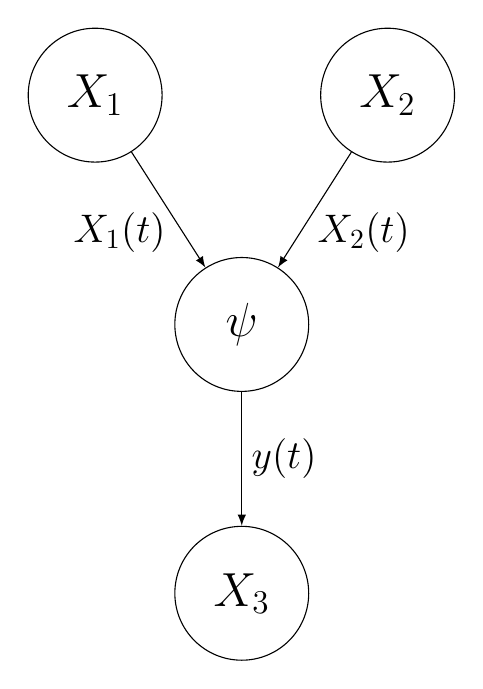
\begin{tikzpicture}
			\tikzstyle{var} = [draw, circle, minimum size=1.7cm]
			\tikzstyle{arrow} = [-latex, line width=0.5pt]
			\tikzstyle{line} = [draw, -latex]
			
			\node [var] (x1) {\LARGE $X_1$};
			\node [var, right=2 cm of x1] (x2) {\LARGE $X_2$};
			\node [var, below right=1.7cm and 0.65cm of x1] (psi) {\LARGE $\psi$};
			\node [var, below=1.7 cm of psi] (x3) {\LARGE $X_3$};
			
			\path [line] (x1)  -- node[pos=0.7, left=.1cm] {\Large$ X_1(t) $} (psi);
			\path [line] (x2)  -- node[pos=0.7, right=.1cm] {\Large$ X_2(t) $} (psi);
			\path [line] (psi)  -- node[midway, right] {\Large$ y(t) $} (x3);
			\end{tikzpicture}
		}
%		\caption{The communication model.}
%		\label{fig:graph_model}
		%	\vspace{-8pt}
%	\end{wrapfigure}
\end{columns}
\end{frame}


\begin{frame}{Graphical Model}
% \vspace{-10pt}
\fontsize{9pt}{6}\selectfont
\begin{columns}[onlytextwidth,c]
	\column{.2\linewidth}
	\centering
	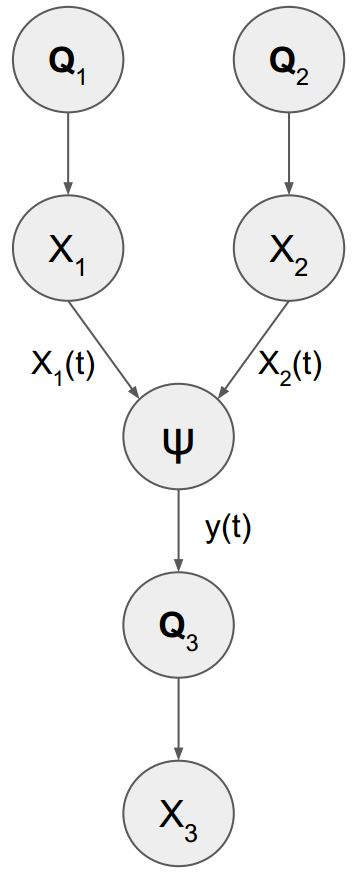
\includegraphics[width=0.75\linewidth]{figures/h_model}
	\column{.8\linewidth}
	\begin{itemize}
		\item $ X_{1} $ and $ X_{2} $ homogenous continuous-time Markov processes with $ \textbf{Q}_{1} $ and $ \textbf{Q}_{2} $ transition intensity matrices
		\vspace{-0.1cm}
		\begin{equation}
		\textbf{Q}_{i} \sim Gam(\alpha_{i}, \beta_{i}),\ \ i \in \left\lbrace 1,2\right\rbrace 
		\end{equation}
		\item $X_{3} $ inhomogeneous continuous-time Markov process  with set of actions $ a \in \left\lbrace a_{0}, a_{1}\right\rbrace  $ and set of transition intensity matrices $ \textbf{\textit{Q}}_{3} = \left\lbrace \textbf{Q}_{a_{0}}, \textbf{Q}_{a_{1}} \right\rbrace  $
		\vspace{-0.1cm}
		\begin{equation}
		\textbf{Q}_{a} \sim Gam(\alpha_{a}, \beta_{a})
		\end{equation}
		\item $ \rchi_{i} = \left\lbrace 0,1\right\rbrace  $
		\item $ \psi  := p(y(t) \mid X_{1}(t), X_{2}(t)) $ observation model\\
		\item $  b(x_{1}, x_{2}; t) $ : belief state
		\item $ \pi(a \mid b) $ : optimal policy of $ X_{3} $
		\item $ X_{i}^{[0,T]} $: discrete valued trajectory in time interval $ [0, T] $
	\end{itemize}
\end{columns}
\end{frame}


\begin{frame}{Problem Statement}
\begin{columns}[onlytextwidth,c]
	\column{.2\linewidth}
	\centering
	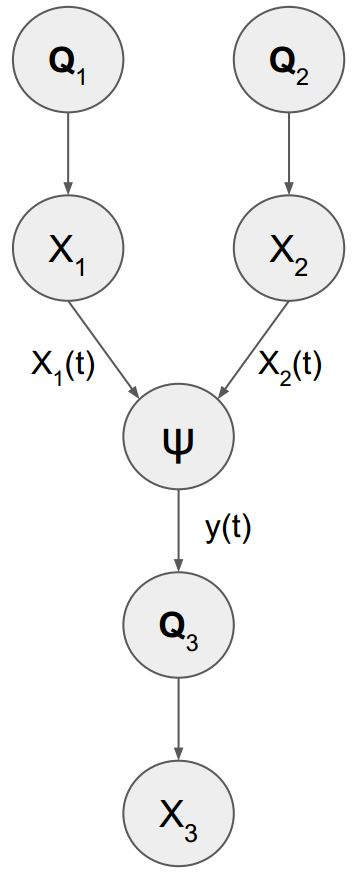
\includegraphics[width=0.75\linewidth]{figures/h_model}
	\column{.8\linewidth}
	\begin{itemize}
		\item While acting in the environment, the agent is assumed to have access to following parameters:
		\begin{itemize}
			\item Transition intensity matrices of the parents $ \textbf{Q}_{1} $ and $ \textbf{Q}_{2} $
			\item Observation model $ \psi $
			\item The optimal policy and $ \textbf{\textit{Q}}_{3} $
		\end{itemize}
		\item For the inference problem, the following parameters are given:
		\begin{itemize}
			\item Transition intensity matrices of the parents $ \textbf{Q}_{1} $ and $ \textbf{Q}_{2} $
			\item The optimal policy and $ \textbf{\textit{Q}}_{3} $
		\end{itemize}
	\end{itemize}
\end{columns}
\end{frame}


\begin{frame}{Belief State $ b(x_{1}, x_{2}; t) $}
\begin{itemize}
	\item Belief state is the probability distribution over state space given the observations
	\begin{equation}
	b(x_{1}, x_{2}; t) = P( X_{1}(t) = x_{1},  X_{2}(t) = x_{2}\mid y_{1}, ..., y_{t})
	\end{equation}
	\item Denote $ b(t) $, $ t \geq 0 $, as row vector with $ \left\lbrace b(x_{1}, x_{2};t)_{x_{i} \in \rchi_{i}}\right\rbrace  $.
	\item This posterior probability can be described by a system of ODEs
	\begin{equation}
	\frac{db(t)}{dt} = b(t)\ \textbf{T}
	\end{equation}
	where the initial condition $ b(0) $ is row vector with $ \left\lbrace P(X_{1}(0)=x_{1}, X_{2}(0)=x_{2})_{x_{i} \in \rchi_{i}}\right\rbrace $ \cite{article}.
	\item \textbf{T} is the joint transition intensity matrix of $ X_{1} $ and $ X_{2} $ and given by amalgamation operation between $ \textbf{Q}_{1} $ and  $ \textbf{Q}_{2} $ \cite{Nodelman1995}.
	\begin{equation}
	\textbf{T} = \textbf{Q}_{1} * \textbf{Q}_{2}
	\end{equation}
\end{itemize}
\end{frame}


\begin{frame}{Belief Update}
\begin{itemize}
	\item The belief update at discrete times of observation $ y_{t} $
	\begin{align}
	b(x_{1}, x_{2}; t) & = P( X_{1}(t) = x_{1},  X_{2}(t) = x_{2}\mid y_{1}, ..., y_{t}) \nonumber\\ & = \frac{P(y_{1}, ..., y_{t}, X_{1}(t) = x_{1},  X_{2}(t) = x_{2})}{P(y_{1}, ..., y_{t})}  \nonumber\\ & = \frac{P(y_{t} \mid y_{1}, ..., y_{t-1}, X_{1}(t) = x_{1},  X_{2}(t) = x_{2})}{P(y_{t} \mid y_{1}, ..., y_{t-1})} \frac{P(y_{1}, ..., y_{t-1}, X_{1}(t) = x_{1},  X_{2}(t) = x_{2})}{P(y_{1}, ..., y_{t-1})}  \nonumber\\ & = Z_{t}^{-1} \ P(y_{t} \mid x_{1}, x_{2})\ P( X_{1}(t) = x_{1},  X_{2}(t) = x_{2}\mid y_{1}, ..., y_{t-1})  \nonumber\\ & = Z_{t}^{-1}\ \textcolor[rgb]{0.16,0.32,0.75}{P(y_{t} \mid x_{1}, x_{2})}\ \textcolor[rgb]{0.8,0,0}{b(x_{1}, x_{2}; t^{-})}
	\end{align}
	where $ Z_{t} = \sum_{x_{1}, x_{2}\in X} P(y_{t} \mid x_{1}, x_{2})\ b(x_{1}, x_{2}; t^{-}) $ is the normalization factor \cite{article}.
\end{itemize}
\end{frame}


\begin{frame}{Inhomogeneous Transition Intensity Matrix $ \textbf{Q}_{3}(t)$}
\begin{itemize}
	\item Let $ \pi(a \mid b) $ be an optimal policy, where $ a \in \left\lbrace a_{0}, a_{1}\right\rbrace  $ is action, and $ \textbf{\textit{Q}}_{3} = \left\lbrace \textbf{Q}_{a_{0}}, \textbf{Q}_{a_{1}} \right\rbrace  $ be a set of intensity matrices of $ X_{3} $ corresponding to each action.
	\item The inhomogeneous transition intensity matrix $ \textbf{Q}_{3}(t) $ can be written as
	\begin{equation}
	\begin{split}
	\textbf{Q}_{3}(t) = \sum_{a} \textbf{Q}_{a}\ \pi(a \mid b(x_{1}, x_{2};t)).
	\end{split}
	\label{eq.Q3}
	\end{equation}
\end{itemize}
\end{frame}


\begin{frame}{Markov Processes}
\begin{itemize}
	\item Consider a homogenous Markov process X with values $ \rchi = \left\lbrace x_{0}, x_{1},..., x_{n}\right\rbrace  $. The transition intensity matrix \textbf{Q} of such process has the following form:
	\begin{equation}
	\textbf{Q} = 
	\begin{bmatrix}
	-q_{x_{0}} & q_{x_{0}x_{1}} & 	{\hdots}  & q_{x_{0}x_{n}} \\
	q_{x_{1}x_{0}} & -q_{x_{1}} & 	{\hdots}  & q_{x_{1}x_{n}}  \\
	{\vdots}  & 	{\vdots}  & 	{\ddots}  & {\hdots}  \\
	 q_{x_{n}x_{0}} &  q_{x_{n}x_{1}} &  {\hdots} & -q_{x_{n}}
	\end{bmatrix}
	\end{equation}
	where $ q_{x} = \sum_{x' \neq x, x' \in \rchi} q_{xx'}$.
	\item The amount of time that X stays in a transitioned state is exponentially distributed, and the probability density function of staying in a state x is given by \cite{Nodelman1995}
	\begin{equation}
	f(t) = q_{x}\ exp(-q_{x}t).
	\end{equation}
\end{itemize}
\end{frame}


\begin{frame}{Likelihood Functions}
\framesubtitle{Homogenous continuous-time Markov process}
\fontsize{9pt}{6}\selectfont
\begin{itemize}
	\item The likelihood of a single transition $ d = \left\langle x,t,x'\right\rangle $, where transition happens from $x$ to $x'$ after spending time amount of time t:
	\begin{equation}
	P(d  \mid \textbf{Q}) = \left( q_{x}\ exp(-q_{x}t) \right) \left( \frac{q_{xx'}}{q_{x}} \right)
	\end{equation}
	\item The likelihood of trajectory $X^{[0,T]}$ can be decomposed as a product of likelihood of single transitions.
	\begin{align}
	P(X^{[0,T]}  \mid \textbf{Q}) & = \left( \prod_{x}  q_{x}^{M[x]}\ exp(-q_{x}T[x]) \right) \left( \prod_{x} \prod_{x' \neq x}  \frac{q_{xx'}}{q_{x}}^{M[x,x']} \right) \nonumber\\ & = \prod_{x}  exp(-q_{x}T[x]) \prod_{x' \neq x}  q_{xx'}^{M[x,x']}
	\label{homo_llh}
	\end{align}
	where $ T[x] $ is the total time spent in state x, $ M[x,x'] $ is the number of transitions from state x to state x', $ M[x] $ is total number of transitions leaving state x \cite{Nodelman2014}.
\end{itemize}
\end{frame}

\begin{frame}{Likelihood Functions}
\framesubtitle{Inhomogeneous continuous-time Markov process}
\begin{itemize}
	\item Similarly, let X be an inhomogeneous Markov process, and \textbf{Q}(t) be the transition intensity matrix. The probability density function of staying in a state x is
	\begin{equation}
	f(t) = q_{x}(t)\ \exp\left( -\int q_{x}(u)du\right)
	\end{equation}
	\item The likelihood of trajectory $X^{[0,T]}$ with $ m $ transitions at $ t_{0}, t_{1}, ..., t_{m} $ \cite{Perez-Ocon2000}

	\begin{align}
	P(X^{[0,T]} \mid \textbf{Q}^{[0,T]}) & = \prod_{k=1}^{m} \left[ q_{x_{k-1}} (t_{k}) \exp \left(-\int_{t_{k-1}}^{t_{k}} q_{x_{k-1}}(u) d u\right) \frac{q_{x_{k-1}, x_{k}} (t_{k})}{q_{x_{k-1}}(t_{k})}\right] \nonumber\\ & =  \prod_{k=1}^{m} \left[q_{x_{k-1}, x_{k}}(t_{k})\ \exp \left(-\int_{t_{k-1}}^{t_{k}} q_{x_{k-1}}(u) d u\right)\right] .
	\end{align}

\end{itemize}
\end{frame}


\begin{frame}{Likelihood Model of the System}
\begin{itemize}
	\item Let \textit{D} be a sample of trajectories in the dataset, such that $ \textit{D} = \left\langle X_{1}^{[0, T]}, X_{2}^{[0, T]}, X_{3}^{[0, T]} \right\rangle  $, and the set of parameters to the system $  \theta = \left\langle \textbf{Q}_{1}, \textbf{Q}_{2}, \textbf{\textit{Q}}_{3}, \pi, \psi \right\rangle  $.
	\item The likelihood of the sample trajectory \textit{D} can be written as

	\begin{align}
	P(\textit{D} \mid \theta ) & = P(X_{1}^{[0, T]}, X_{2}^{[0, T]}, X_{3}^{[0, T]} \mid \textbf{Q}_{1}, \textbf{Q}_{2}, \textbf{\textit{Q}}_{3}, \pi, \psi) \nonumber\\ & = P(X_{3}^{[0, T]} \mid X_{1}^{[0, T]}, X_{2}^{[0, T]}, \textbf{Q}_{1}, \textbf{Q}_{2}, \textbf{\textit{Q}}_{3}, \pi, \psi) \ P(X_{1}^{[0, T]}\mid \textbf{Q}_{1}) \ P(X_{2}^{[0, T]}\mid \textbf{Q}_{2}) \nonumber\\ & = P(X_{3}^{[0, T]}\mid \textbf{ Q}_{3}^{[0, T]}) \ P(X_{1}^{[0, T]}\mid \textbf{Q}_{1}) \ P(X_{2}^{[0, T]}\mid \textbf{Q}_{2}) 
	\end{align}

	where $ \textbf{Q}_{3}^{[0, T]} $ is a deterministic function of $X_{1}^{[0, T]}, X_{2}^{[0, T]}, \textbf{Q}_{1}, \textbf{Q}_{2}, \textbf{\textit{Q}}_{3}, \pi $ and $ \psi $, given by Eq.\ref{eq.Q3}.
\end{itemize}
\end{frame}


%%\begin{frame}{Likelihood model of the communication system}
%%\begin{itemize}
%%	\item Marginalizing the likelihood over $ \textbf{Q}_{1} $ and $ \textbf{Q}_{2} $:
%%	\begin{equation}
%%	\begin{split}
%%	P(\textit{D} \mid \pi, \phi ) & = 	\int \int P(\textit{D} \mid \theta ) \ P(\textbf{Q}_{1}) \ P(\textbf{Q}_{2}) \ d\textbf{Q}_{1}d\textbf{Q}_{2} \\ & = \int \int P(X_{3}^{[0, T]}\mid \textbf{Q}_{3}^{[0, T]}) \ P(X_{1}^{[0, T]}\mid \textbf{Q}_{1}) \ P(X_{2}^{[0, T]}\mid \textbf{Q}_{2}) \ P(\textbf{Q}_{1}) \ P(\textbf{Q}_{2})\ d\textbf{Q}_{1}d\textbf{\textbf{Q}}_{2} \\ & = P(X_{3}^{[0, T]}\mid \textbf{Q}_{3}^{[0, T]}) \int  P(X_{1}^{[0, T]}\mid \textbf{Q}_{1}) \ P(\textbf{Q}_{1}) \ d\textbf{Q}_{1} \int P(X_{2}^{[0, T]}\mid \textbf{Q}_{2})\ P(\textbf{Q}_{2})\ d\textbf{Q}_{2}
%%	\label{eq:Marg_llh}
%%	\end{split}
%%	\end{equation}
%%\end{itemize}
%%\end{frame}
%
%%
%%\begin{frame}{Likelihood model of the communication system}
%%\framesubtitle{Marginal probability of a trajectory of homogenous Markov Process}
%%\begin{itemize}
%%	\item 	Let X be a homogenous binary-valued Markov process.
%%	\item The transition intensity matrix \textbf{Q} can be written in the following form for convenience,
%%	\begin{equation}
%%		\textbf{Q} = 
%%		\begin{pmatrix}
%%		-q_{0} & q_{0} \\
%%		q_{1} & -q_{1}
%%		\end{pmatrix}
%%	\end{equation}
%%	where the transition intensities $ q_{0} $ and $ q_{1} $ are gamma-distributed with parameters $ \alpha_{0}$, $ \beta_{0} $ and $ \alpha_{1} $, $ \beta_{1} $, respectively.
%%\end{itemize}
%%\end{frame}
%
%
%%\begin{frame}[shrink=20]{Likelihood model of the communication system}
%%\framesubtitle{Marginal probability of a trajectory of homogenous Markov Process}
%%\vspace{-0.5cm}
%%	\begin{equation}
%%	\begin{split}
%%	P(X^{[0, T]}) & = \int  P(X^{[0, T]}\mid \textbf{Q})P(\textbf{Q}) d\textbf{Q} \\ & = \int_{0}^{\infty} \left( \prod_{x} \exp(-q_{x}T_{x}) \prod_{x'} q_{xx'}^{M[x, x']}\right) \frac{\beta_{xx'}^{\alpha_{xx'}}{q_{xx'}^{\alpha_{xx'}-1}}\exp(-\beta_{xx'}q_{xx'})}{\Gamma(\alpha_{xx'})} \ dq_{xx'} \\ & = \prod_{x\in{0,1}}\int_{0}^{\infty} q_{x}^{M_{x}} \ \exp(-q_{x}T_{x}) \  \frac{\beta_{x}^{\alpha_{x}} \ q_{x}^{\alpha_{x}-1}\ \exp(-\beta_{x}q_{x})}{\Gamma(\alpha_{x})} \ dq_{x} \\ & = \prod_{x\in{0,1}} \frac{\beta_{x}^{\alpha_{x}}}{\Gamma(\alpha_{x})} \int_{0}^{\infty} q_{x}^{M_{x} + \alpha_{x} -1} \ \exp(-q_{x}(T_{x}+\beta_{x})) \ dq_{x} \\ & = \prod_{x\in{0,1}} \frac{\beta_{x}^{\alpha_{x}}}{\Gamma(\alpha_{x})} \left( -(T_{x}+\beta_{x})^{M_{x} + \alpha_{x}}\ \Gamma(M_{x} + \alpha_{x}, \ q_{x}(T_{x}+\beta_{x})) \right) \Big|_0^\infty  \\ & = \prod_{x\in{0,1}} \frac{\beta_{x}^{\alpha_{x}}}{\Gamma(\alpha_{x})} \left( (T_{x}+\beta_{x})^{M_{x} + \alpha_{x}}\ \Gamma(M_{x} + \alpha_{x}) \right)
%%	\label{eq:Marg_traj}
%%	\end{split}
%%	\end{equation}
%%	where $ T_{x} $, the amount of time spent in state x, $ M[x,x'] $ the number of transitions from state x to x' and  $ M[x] = \sum_{x\neq x'}M[x,x'] $.
%%\end{frame}
%
%%
%%\begin{frame}{Likelihood model}
%%\framesubtitle{Overall system}
%%\begin{itemize}
%%	\item Plugging Eq.\ref{eq:Marg_traj} in Eq.\ref{eq:Marg_llh} for both $ X_{1} $ and $ X_{2} $:
%%	\begin{align}
%%	\begin{split}
%%	P(\textit{D} \mid \pi, \phi ) = P(X_{3}^{[0, T]}\mid \textbf{Q}_{3}^{[0, T]}) \prod_{x_{1}\in{0,1}} \frac{\beta_{x_{1}}^{\alpha_{x_{1}}}}{\Gamma(\alpha_{x_{1}})} \ (T_{x_{1}}+\beta_{x_{1}})^{M_{x_{1}} + \alpha_{x_{1}}}\ \Gamma(M_{x_{1}} + \alpha_{x_{1}})  \\  \prod_{x_{2}\in{0,1}} \frac{\beta_{x_{2}}^{\alpha_{x_{2}}}}{\Gamma(\alpha_{x_{2}})} \ (T_{x_{2}}+\beta_{x_{2}})^{M_{x_{2}} + \alpha_{x_{2}}}\ \Gamma(M_{x_{2}} + \alpha_{x_{2}})
%%	\label{eq:Marg_llh_final}
%%	\end{split}
%%	\end{align}
%%\end{itemize}
%%\end{frame}
%%
%
\begin{frame}{Simulation and Results}
\framesubtitle{Parameters}
\begin{columns}[T]
	\column{.5\linewidth}
	\begin{itemize}
		\item Intensity matrices \\
		$ \textbf{Q}_{1} = 
		\begin{bmatrix} \vspace{-2pt}
		-3.2 & 3.2 \\  \vspace{-2pt}
		0.5 & -0.5 
		\end{bmatrix} $\\
		\vspace{+3pt}
		 $ \textbf{Q}_{2} = 
		\begin{bmatrix} \vspace{-2pt}
		-1.5 & 1.5 \\  \vspace{-2pt}
		3.45 & -3.45
		\end{bmatrix}$\\
		\vspace{+3pt}
		$\textbf{\textit{Q}}_{3} = \left\lbrace 
		\begin{bmatrix} \vspace{-2pt}
		-0.5 & 0.5 \\  \vspace{-2pt}
		25 & 25 
		\end{bmatrix}, 
		\begin{bmatrix} \vspace{-2pt}
		-32 & 32 \\  \vspace{-2pt}
		0.02 & -0.02 
		\end{bmatrix} \right\rbrace $
	\end{itemize}
	\column{.5\linewidth}
	\begin{itemize}
		\item Observation models \vspace{+4pt} \\
		$\psi_{0} =
		\begin{bmatrix} \vspace{-2pt}
		1 & 0 & 0 \\  \vspace{-2pt}
		0 & 1 & 0 \\  \vspace{-2pt}
		0 & 1 & 0 \\  \vspace{-1pt}
		0 & 0 & 1
		\end{bmatrix}$\\
 		\vspace{+6pt}
		$\psi_{1} = 
		\begin{bmatrix} \vspace{-2pt}
		0 & 0 & 1 \\  \vspace{-2pt}
		0 & 1 & 0 \\  \vspace{-2pt}
		1 & 0 & 0 \\  \vspace{-1pt}
		0 & 0 & 1 
		\end{bmatrix} $\\
		\vspace{+6pt}
		$\psi_{2} = 
		\begin{bmatrix} \vspace{-2pt}
		0 & 0 & 1 \\  \vspace{-2pt}
		1 & 0 & 0 \\  \vspace{-2pt}
		0 & 0 & 1 \\  \vspace{-1pt}
		0 & 1 & 0  
		\end{bmatrix}$
	\end{itemize}
\end{columns}
\end{frame}

\begin{frame}{Simulation}
\framesubtitle{Sampling trajectories using Gillespie algorithm}
\begin{itemize}
	\item Sampled trajectory example:
	\begin{tabular}{cc}
		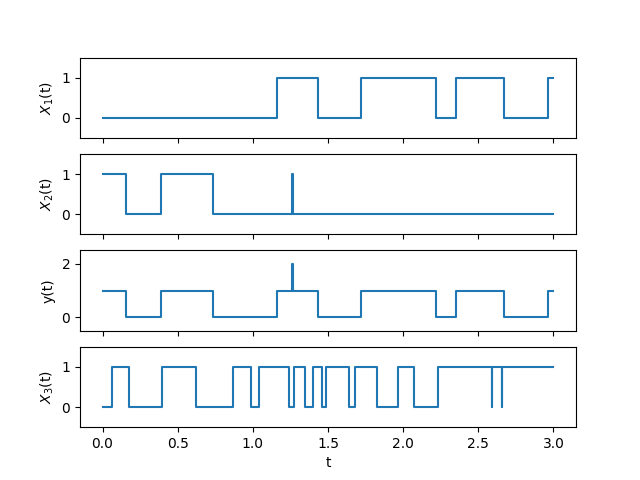
\includegraphics[height=0.66\textheight]{figures/trajectory_plot}
		&
		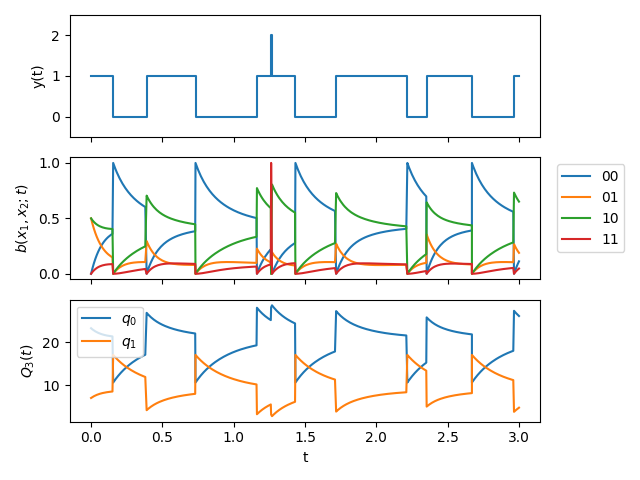
\includegraphics[height=0.6\textheight]{figures/b_Q_plot}
	\end{tabular}
\end{itemize}
\end{frame}


\begin{frame}{Results}
\framesubtitle{Maximum likelihood estimation}
\begin{columns}[onlytextwidth,c]
	\column{.5\linewidth}
	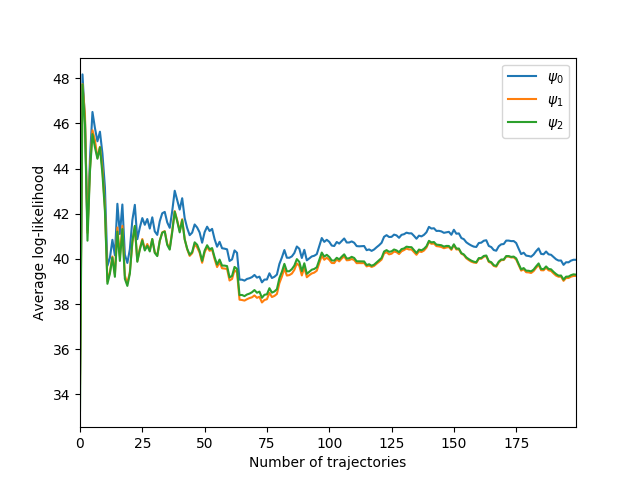
\includegraphics[width=\linewidth]{figures/llh_}
	\column{.5\linewidth}
	\begin{itemize}
		\item Observation models \vspace{+4pt} \\
		$\psi_{0} =
		\begin{bmatrix} \vspace{-2pt}
		1 & 0 & 0 \\  \vspace{-2pt}
		0 & 1 & 0 \\  \vspace{-2pt}
		0 & 1 & 0 \\  \vspace{-1pt}
		0 & 0 & 1
		\end{bmatrix}$\\
		\vspace{+6pt}
		$\psi_{1} = 
		\begin{bmatrix} \vspace{-2pt}
		0 & 0 & 1 \\  \vspace{-2pt}
		0 & 1 & 0 \\  \vspace{-2pt}
		1 & 0 & 0 \\  \vspace{-1pt}
		0 & 0 & 1 
		\end{bmatrix} $\\
		\vspace{+6pt}
		$\psi_{2} = 
		\begin{bmatrix} \vspace{-2pt}
		0 & 0 & 1 \\  \vspace{-2pt}
		1 & 0 & 0 \\  \vspace{-2pt}
		0 & 0 & 1 \\  \vspace{-1pt}
		0 & 1 & 0  
		\end{bmatrix}$
	\end{itemize}
\end{columns}
\end{frame}


\begin{frame}{Results}
\framesubtitle{Receiver Operating Characteristic(ROC) Analysis}
\begin{columns}[onlytextwidth,c]
	\column{.5\linewidth}
	\centering
	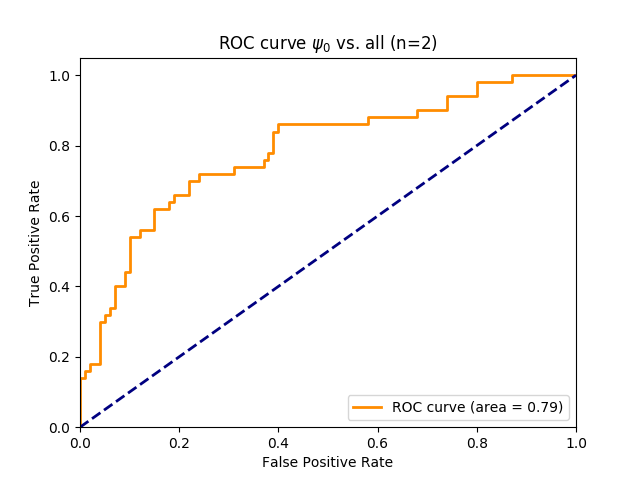
\includegraphics[width=\linewidth]{figures/AUROC_100samples_class0_llh_n2}
	\column{.5\linewidth}
	\begin{itemize}
		\item Classification problem between same observation models
		\item 300 trajectories, class-balanced
	\end{itemize}
\end{columns}
\end{frame}


\begin{frame}{Conditional Intensity Marginalization}
\framesubtitle{over $ \textbf{Q}_{1} $ and $ \textbf{Q}_{2} $}
\begin{itemize}
	\item Replacing the exact belief update with marginal particle filter approximation
	\begin{itemize}
		\item Removing the assumption that transition intensity matrices of $ X_{1} $ and $ X_{2} $ are available to agent $ X_{3} $
		\item More realistic system
	\end{itemize}
	\item Given the priors and sample trajectory, the intensity matrices can be replaced by estimates. \cite{Studer2016}
	\begin{itemize}
		\item $\textbf{Q}_{i}$ with non-diagonal entries $ q^{i}_{xx'}\sim Gam(\alpha_{i}\left(x, x^{\prime}\right), \beta_{i}\left(x, x^{\prime}\right)),\ \ i \in \left\lbrace 1,2\right\rbrace $
		\item $X_{i}^{[0,T]}$ with summary statistics $ T_{i}[x] $ and $ M_{i}[x,x'] $, where $ T_{i}[x] $ is the total time spent in state x, $\ M_{i}[x,x'] $ is the number of transitions from state x to state x'
		\item Using Bayes' rule and the likelihood of trajectory in Eq.\ref{homo_llh}, the estimates can be evaluated analytically as follows:
		\begin{equation}
		E\left[ q^{i}_{xx'} | X^{[0,T]}\right]=\frac{\alpha_{i}\left(x, x^{\prime}\right)+M_{i}\left[x, x^{\prime}\right]}{\beta_{i}\left(x, x^{\prime}\right)+T_{i}[x]}
		\end{equation}
	\end{itemize}
\end{itemize}
\end{frame}


\begin{frame}{Marginal Particle Filter}
\begin{itemize}
	\vspace{-5pt}
	\item Given a prior distribution over states, the particles are initialized $ \textbf{p}^{0} $.
\end{itemize}
\scalebox{1}{\begin{algorithm}[H]
	\KwIn{Measurement data $ y_{k} $ at time $ t_{k} $, set of particles $ \textbf{p}^{k-1} $}
	\KwResult{New set of particles $ \textbf{p}^{k} $, representing $ b(t_{k}) $}
	\vspace{+4pt}
	\begin{algorithmic}[1]
		\FOR{$p_{m} \in \textbf{p}^{k-1}$}
		\STATE {$p_{m} = \left\lbrace x_{m}, \textbf{T}_{m}, \textbf{M}_{m}\right\rbrace \leftarrow Propagate\ particle\ through\ marginal\ process\ model\ from\ t_{k-1}\ to\ t_{k}$ }
		\STATE{$w_{m} \leftarrow p(y_{k} \mid X(t_{k})=x_{m}) $} 
		\tcp*[h] {observation likelihood}
		\ENDFOR
		\STATE{$ w_{m} \leftarrow \frac{w_{m}}{\sum_{m} w_{m}}$} \tcp*[h]{normalize weights}
		\FOR{$ p_{m} \in \textbf{p}_{k} $} 
		\STATE{$ p_{m} \leftarrow Sample\ from\ p_{k}\ with\ probabilities\ w_{m}\ with\ replacement$}
		\ENDFOR
	\end{algorithmic}
	\caption{Marginal particle filter\cite{Studer2016}}
	\label{alg:seq}
\end{algorithm}}
\end{frame}


\begin{frame}{Future work}
\begin{itemize}
	\item Implementation of marginal particle filter
	\item Application on real-world data
	\begin{itemize}
	\item e.g. British Household Panel Survey
	\end{itemize}
	\item Inference of observation model in an interactive multi-agent system
\end{itemize}
\vspace{+.5cm}
\centering
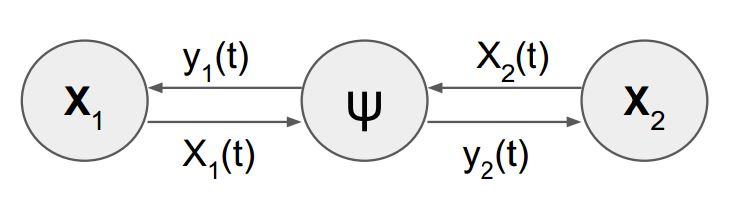
\includegraphics[width=0.4\linewidth]{figures/multi-agent}
\end{frame}
 

\begin{frame}{References}
\vspace{-5pt}
\small
\bibliographystyle{ieeetr}
\bibliography{bib_cleaned}
\end{frame}


\begin{frame}[c]{}
\centering \Huge
Thank you!
\end{frame}


\begin{frame}{Backup}
\framesubtitle{ROC Analysis}
\begin{columns}[t]
	\column{.33\textwidth}
	\centering
	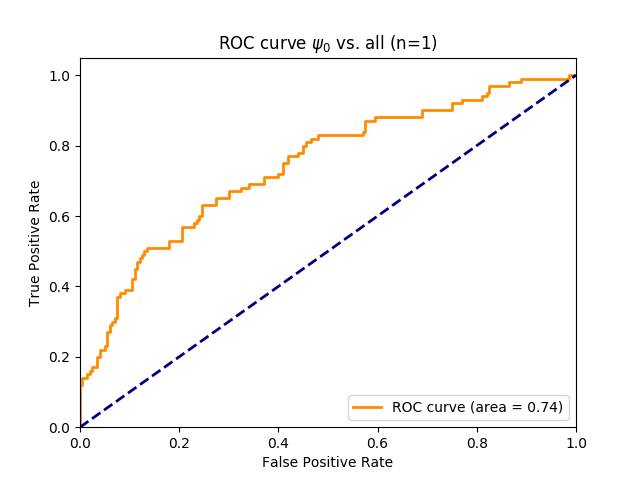
\includegraphics[width=4cm,height=2.7cm]{figures/AUROC_100samples_class0_llh_n1}\\
	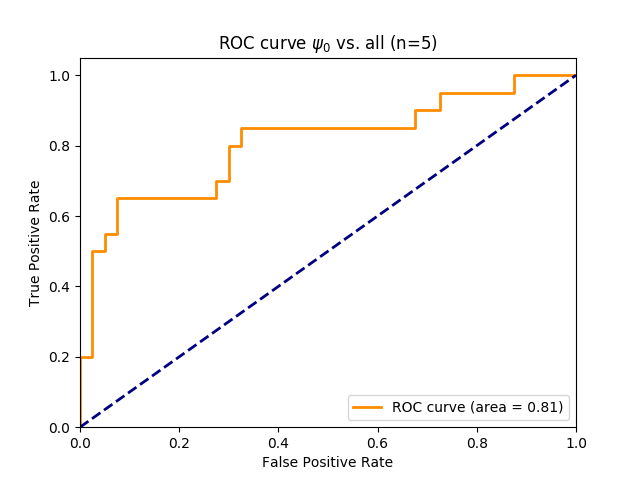
\includegraphics[width=4cm,height=2.7cm]{figures/AUROC_100samples_class0_llh_n5}
	\column{.33\textwidth}
	\centering
	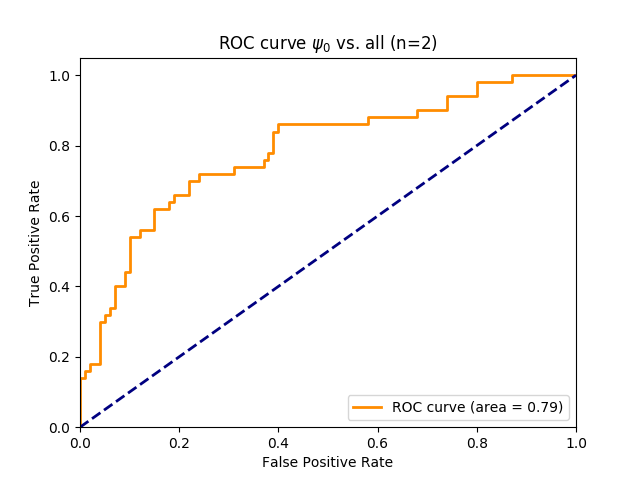
\includegraphics[width=4cm,height=2.7cm]{figures/AUROC_100samples_class0_llh_n2}\\
	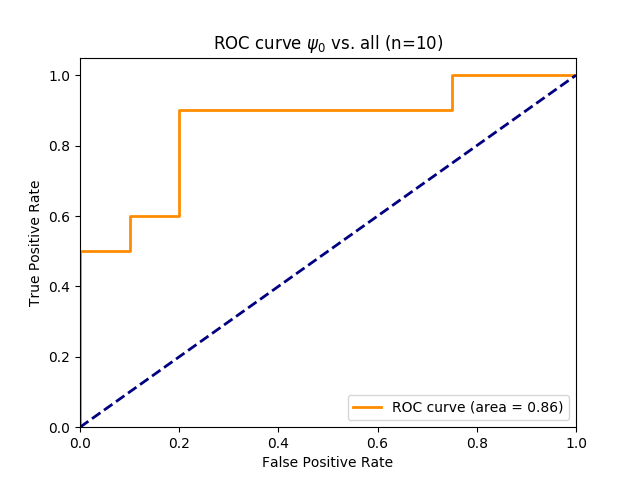
\includegraphics[width=4cm,height=2.7cm]{figures/AUROC_100samples_class0_llh_n10}
	\column{.33\textwidth}
	\centering
	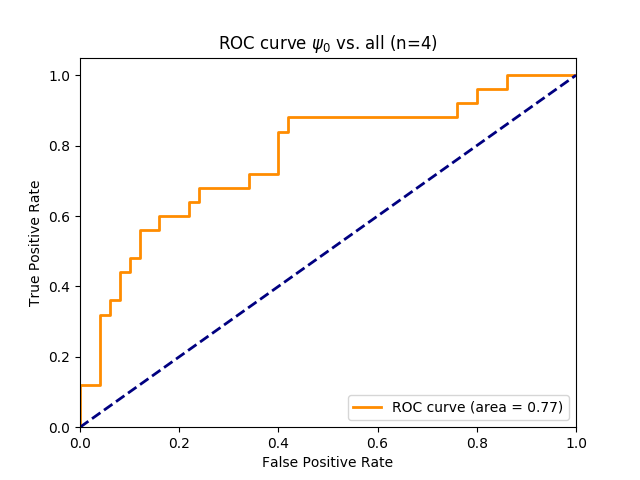
\includegraphics[width=4cm,height=2.7cm]{figures/AUROC_100samples_class0_llh_n4}\\
	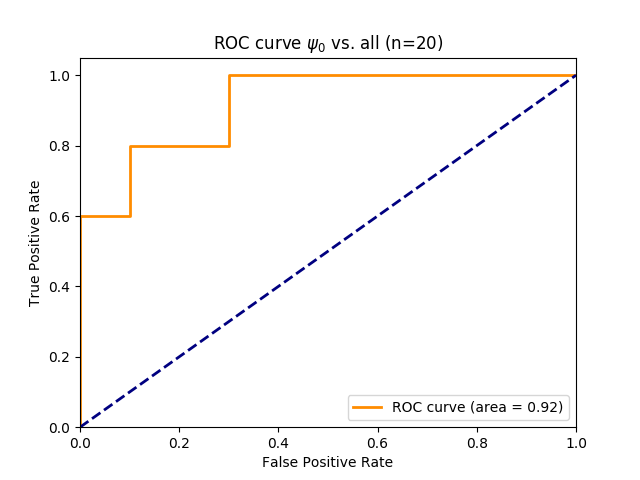
\includegraphics[width=4cm,height=2.7cm]{figures/AUROC_100samples_class0_llh_n20}
\end{columns}
\end{frame}


\begin{frame}{Backup}
\framesubtitle{MLE}
\centering
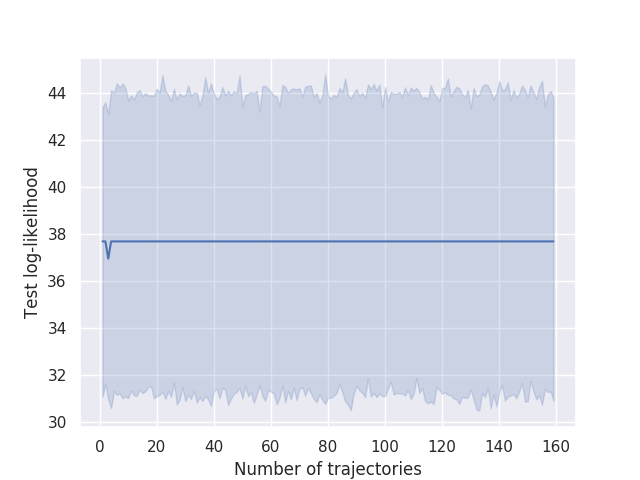
\includegraphics[width=7.5cm,height=5.5cm]{figures/test_likelihood}
\end{frame}

\end{document}